\chapter{Data}
The data was provided by a competition on the website Kaggle for
identifying various types of comments~\cite{toxic-kaggle}. It contains
Wikipedia comments in plain text together with labels indicating toxic
behaviour.

\begin{table}[H]
  \centering
  \caption{Example comments with their labels.}    
  \label{tbl:comments}
  \resizebox{14cm}{!}{%
    \begin{tabular}{l|lccccc}
      Comment &  severe toxic &  obscene &  threat &  insult &  identity                                                         hate \\
      \hline
      "\textbackslash n Sure, but the lead must... &             0 &        0 &       0 &       0 &              0 \\
      TFD \textbackslash n\textbackslash nI think we just eced. I... &             0 &        0 &       0 &       0 &              0 \\
      You are gay or antisemmitian? \textbackslash... &             0 &        1 &       0 &       1 &              1 \\
      FUCK YOUR FILTHY MOTHER IN... &             0 &        1 &       0 &       1 &              0 \\
      I'm Sorry \textbackslash n\textbackslash nI'm sorry I... &             0 &        0 &       0 &       0 &              0 \\
      I don't believe the Lisak critic... &             0 &        0 &       0 &       0 &              0 \\
      You had a point, and it's now am... &             0 &        0 &       0 &       0 &              0 \\
      In other words, you're too lazy to... &             0 &        0 &       0 &       0 &              0 \\
      "\textbackslash nAs for your claims of ""stalking""... &             0 &        0 &       0 &       0 &              0 \\
      "::::Jmabel; in regards to predomin... &             0 &        0 &       0 &       0 &              0 \\
    \end{tabular}
  }
\end{table}
The different labels of the comments were ``toxic'', ``severe toxic'' ,
``obscene'', ``threat'', ``insult'',  ``identity'', and ``hate''. Some
truncated comments and their labels can be seen in
Table~\ref{tbl:comments}. 
\begin{figure}[H]
  \centering
  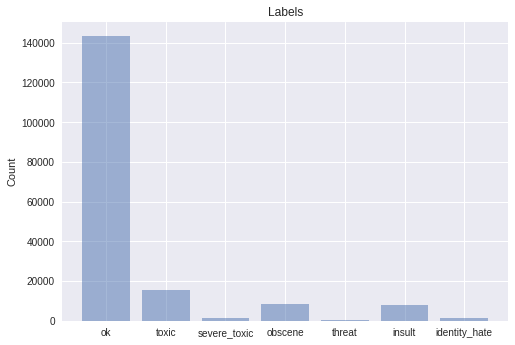
\includegraphics[width=0.8\textwidth]{graphics/label-dist}
  \caption{The count of different labels. Since labels are independent,
    one comment can contribute to several label counts.}\label{fig:labels-dist}
\end{figure}
As suggested by the table, the data was skewed towards
unflagged comments. Figure~\ref{fig:labels-dist} show the counts of the
different labels, where it can be seen that the labels ``severe
toxic'', ``threat'' and ``identity hate'' are increadibly uncommon.
\begin{figure}[H]
  \centering
  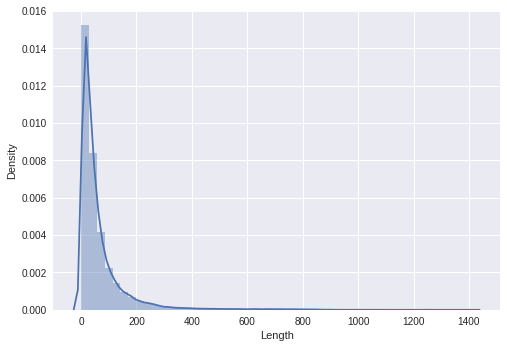
\includegraphics[width=0.8\textwidth]{graphics/comment-word-count}
  \caption{Density plot of comment word counts.}\label{fig:comment-word-count}
\end{figure}
Plotting the word count of the comments show that almost all comments
have less than 200 words in them.